\documentclass[conference]{IEEEtran}
\usepackage{cite}
\usepackage{amsmath,amssymb,amsfonts}
\usepackage{algorithmic}
\usepackage{graphicx}
\usepackage{textcomp}
\usepackage{xcolor}
\usepackage[indonesian]{babel}
\addto\captionsindonesian{\renewcommand{\abstractname}{Abstrak}\renewcommand{\refname}{Daftar Pustaka}}
\renewcommand{\IEEEkeywordsname}{Kata Kunci}
\graphicspath{{figures/}}

\begin{document}

\title{Analisis Trade-off antara Akurasi dan Efisiensi Komputasi dalam Deteksi Sarkasme Menggunakan DistilBERT dan RoBERTa}

\author{\IEEEauthorblockN{Falah Razan Hibrizi}
\IEEEauthorblockA{\textit{Fakultas Informatika} \\
\textit{Universitas Telkom}\\
Bandung, Indonesia \\
alamat email}
\and
\IEEEauthorblockN{Nama Pembimbing}
\IEEEauthorblockA{\textit{Fakultas Informatika} \\
\textit{Universitas Telkom}\\
Bandung, Indonesia \\
alamat email}
}

\maketitle

\begin{abstract}
Sarkasme sering menyatakan maksud yang berlawanan dengan arti harfiahnya, sehingga sistem analisis sentimen kerap salah membacanya. Penelitian ini mengkaji trade-off antara performa dan efisiensi komputasi RoBERTa dan DistilBERT menggunakan 1.000.864 pasangan comment dan parent comment dari Self-Annotated Reddit Corpus (SARC). Perbandingan mencakup tiga konfigurasi input, yaitu comment saja, early fusion, dan late fusion, serta pembekuan sebagian layer. Konfigurasi final dipilih dari data validasi dan dikunci sebelum skor data uji dihitung. Setiap konfigurasi dijalankan dengan tiga seed dan diuji dengan paired t-test, Wilcoxon signed-rank test, dan Friedman test dengan koreksi Holm. Macro-F1 tertinggi sebesar 79,62\% diperoleh RoBERTa dengan early fusion, dan RoBERTa unggul 1,65--2,07 poin dibanding DistilBERT. Meski begitu, DistilBERT mencapai 97--98\% macro-F1 RoBERTa dengan waktu training, latensi, dan memori GPU sekitar setengahnya. Parent comment menaikkan macro-F1 sebesar 0,69--1,10 poin, terutama pada comment yang ambigu. Pada RoBERTa, early fusion lebih akurat dan jauh lebih hemat daripada late fusion. Pembekuan 6 dari 12 layer RoBERTa hanya mengurangi macro-F1 sebesar 0,24 poin dan memangkas waktu training sekitar 45\%, tetapi latensi inferensi tidak turun. RoBERTa lebih tepat bila akurasi diutamakan, sedangkan DistilBERT lebih tepat bila latensi dan memori terbatas.
\end{abstract}

\begin{IEEEkeywords}
DistilBERT, deteksi sarkasme, efisiensi komputasi, parent comment, pembekuan layer, RoBERTa
\end{IEEEkeywords}

\section{Pendahuluan}
Dalam sarkasme, penutur mengatakan sesuatu yang berlawanan dengan maksud sebenarnya, misalnya memakai pujian untuk mengejek. Kalimat semacam ini sulit ditangani sistem analisis sentimen karena kata yang terlihat positif ternyata bermaksud negatif \cite{prakash2025sarcasm}. Akibatnya, pemantauan opini publik dan moderasi konten dapat keliru, termasuk dalam deteksi perundungan siber di media sosial \cite{dhumpati2025sarcasm}, \cite{grover2026emoji}.

Pada teks tertulis tidak ada nada suara maupun ekspresi wajah sebagai petunjuk \cite{jimenez2026bert}. Di Reddit, sifat sarkas sebuah balasan sering baru terlihat setelah pembaca mengetahui komentar yang dibalas, yang disebut parent comment. Self-Annotated Reddit Corpus (SARC) \cite{khodak2018sarc} menyediakan pasangan parent comment dan balasan dalam jumlah sangat besar. Konteks lain, seperti informasi pengguna dan topik forum, juga membantu model pada SARC \cite{hao2023enhanced}, dan memasukkan parent comment ke model transformer dilaporkan dapat menaikkan performa \cite{ataeii2020transformers}, \cite{dubey2025unpacking}.

RoBERTa \cite{liu2019roberta} merupakan pengembangan BERT dengan prosedur pralatih yang diperbaiki. Akurasinya umumnya tinggi, tetapi kebutuhan memori dan waktu komputasinya besar, padahal sumber daya komputasi terbatas \cite{treviso2023efficient}. DistilBERT \cite{sanh2019distilbert} dihasilkan melalui distilasi pengetahuan sehingga jumlah layernya tinggal setengah dan inferensinya lebih cepat. Studi yang membandingkan varian BERT untuk deteksi sarkasme menunjukkan bahwa performa sangat bergantung pada pilihan model dan pengaturan training \cite{jimenez2026bert}, \cite{ullah2026advanced}.

Dubey dkk.\ membandingkan RoBERTa dan DistilBERT, termasuk pada SARC, dan melaporkan training DistilBERT sekitar 1,74 kali lebih cepat dengan performa yang bersaing \cite{dubey2025unpacking}, \cite{dubey2026efficient}. Akan tetapi, kedua model digabung dengan ringkasan konteks BART dan embedding metadata, eksperimennya hanya memakai subset 7.370 sampel \cite{dubey2025unpacking}, dan prapemrosesannya membuang huruf kapital serta tanda baca yang dapat menjadi petunjuk sarkasme \cite{dubey2026efficient}. Selisih kedua model pada \cite{dubey2026efficient} juga tidak signifikan ($p = 0{,}064$). Zhang dkk.\ \cite{zhang2025enhancing} memakai SARC berskala lebih besar, tetapi tidak memisahkan data uji dari data validasi. Selain itu, cara memasukkan parent comment dan pembekuan layer masih jarang dibahas bersama biaya komputasinya.

Oleh karena itu, penelitian ini membandingkan performa dan efisiensi komputasi RoBERTa dan DistilBERT pada sekitar satu juta pasangan comment SARC tanpa komponen tambahan, lalu menganalisis trade-off keduanya melalui tiga pertanyaan penelitian berikut.
\begin{enumerate}
\item Apakah jumlah layer yang dibekukan memiliki pengaruh terhadap performa klasifikasi sarkasme?
\item Apakah pemanfaatan parent comment sebagai input memiliki pengaruh terhadap performa klasifikasi sarkasme?
\item Strategi fusion seperti apa yang mampu memberikan performa terbaik dalam klasifikasi sarkasme?
\end{enumerate}
Setiap pertanyaan dijawab untuk kedua model dengan mempertimbangkan waktu training, latensi inferensi, memori GPU, dan jumlah parameter. Kontribusi penelitian ini adalah (i) perbandingan dengan prapemrosesan ringan, konfigurasi yang dikunci sebelum data uji dibuka, tiga seed, dan uji statistik dengan koreksi Holm; (ii) pengukuran biaya komputasi untuk tiga input dan beberapa tingkat pembekuan layer; dan (iii) analisis jenis comment yang paling terbantu oleh parent.

\section{Metode}

\subsection{Dataset dan Prapemrosesan}
\label{sec:data}
Penelitian ini memakai SARC \cite{khodak2018sarc} versi seimbang dari Kaggle, sama dengan \cite{dubey2026efficient}, \cite{zhang2025enhancing}, yang berisi 1.010.826 pasangan comment dan parent comment. Labelnya berasal dari penanda ``/s'' yang ditambahkan penulis comment, dan penanda ini sudah dihapus dari teks \cite{khodak2018sarc}.

Berbeda dengan \cite{dubey2026efficient}, \cite{zhang2025enhancing} yang mengubah teks ke huruf kecil, menghapus tanda baca, dan melakukan lematisasi, prapemrosesan di sini dibuat ringan karena huruf kapital, tanda baca, dan emotikon seperti ``;)'' dapat menjadi penanda sarkasme. Pembersihan hanya meliputi dekode entitas HTML, penggantian tautan Markdown dengan teksnya, penghapusan URL dan tag HTML, serta perapian spasi, sehingga hanya 2.942 comment (0,29\%) yang berubah.

Tahap penyaringan ditampilkan pada Tabel~\ref{tab:data}. Duplikat dan label bertentangan dicari dengan kunci yang dinormalisasi (huruf kecil, tanpa tanda baca), tetapi model tetap menerima teks asli. Tahap terakhir membuang sisa penghapusan ``/s'' berupa potongan kalimat seperti ``You forgot the'', yang dicari dengan pola maksimal delapan kata. Dari 8.599 baris yang cocok, 8.580 berlabel sarkas, sehingga semuanya dihapus agar model tidak belajar dari jalan pintas ini. Hasilnya 1.000.864 pasangan dengan proporsi sarkas 49,59\%.

\begin{table}[t]
\caption{Penyaringan Baris dan Pembagian Data}
\label{tab:data}
\centering
\begin{tabular}{lrr}
\hline
Tahap penyaringan & Dibuang & Sisa \\
\hline
Data mentah & -- & 1.010.826 \\
Comment kosong & 55 & 1.010.771 \\
Kosong setelah dibersihkan & 9 & 1.010.762 \\
Label bertentangan & 142 & 1.010.620 \\
Pasangan duplikat & 1.157 & 1.009.463 \\
Potongan ``/s'' & 8.599 & 1.000.864 \\
\hline
Bagian data & Pasangan & Sarkas (\%) \\
\hline
Latih & 799.459 & 49,66 \\
Validasi & 100.276 & 49,38 \\
Uji & 101.129 & 49,27 \\
\hline
\end{tabular}
\end{table}

Data dibagi dengan seed 42 berdasarkan kelompok comment, bukan per baris, karena balasan pendek seperti ``Source?'' muncul ratusan kali. Hasilnya mendekati rasio 80/10/10 tanpa comment maupun pasangan yang muncul di lebih dari satu bagian.

\subsection{Model dan Konfigurasi Input}
RoBERTa-base \cite{liu2019roberta} memiliki 12 layer, ukuran hidden 768, dan 124,6 juta parameter, sedangkan DistilBERT \cite{sanh2019distilbert} memiliki enam layer dan 65,8 juta parameter. Versi cased dipilih untuk DistilBERT agar kedua model dapat membedakan huruf kapital. Tiga konfigurasi input dibandingkan.

\textit{Comment saja.} Model hanya menerima teks balasan sebagai baseline.

\textit{Early fusion.} Parent dan comment disatukan dengan format pasangan kalimat tokenizer, dengan parent di depan, serupa dengan \cite{ataeii2020transformers}, sehingga token comment dapat memperhatikan semua token parent sejak layer pertama. Panjang input dibatasi 256 token dengan memotong akhir parent, yang terjadi pada 0,85\% pasangan latih RoBERTa dan 0,99\% DistilBERT. Comment yang melebihi 256 token hanya 52--54 (kurang dari 0,01\%).

\textit{Late fusion.} Parent dan comment di-encode terpisah dengan encoder yang sama. Hidden state akhir token pertama comment ($h_x$) dan parent ($h_y$) digabung menjadi
\begin{equation}
u = [\,h_x;\; h_y;\; |h_x - h_y|;\; h_x \odot h_y\,],
\label{eq:fusion}
\end{equation}
dengan $[\cdot\,;\cdot]$ penggabungan vektor dan $\odot$ perkalian per elemen. Vektor $u$ pada (\ref{eq:fusion}) diteruskan ke head klasifikasi bawaan model dengan ukuran input empat kali lebih besar. Akibatnya, encoder dijalankan dua kali per contoh dan token comment tidak dapat memperhatikan token parent secara langsung.

\subsection{Pembekuan Layer}
Pembekuan layer termasuk fine-tuning selektif karena hanya sebagian parameter yang dilatih \cite{han2024peft}, dan dapat menghemat memori GPU dengan penurunan akurasi kecil \cite{ardakani2024slimfit}. Embedding layer dan sejumlah layer terbawah dibekukan pada early fusion, yaitu 0, 6, 9, dan 12 dari 12 layer RoBERTa serta 0, 3, dan 6 dari 6 layer DistilBERT. Model yang dibekukan sebagian memakai learning rate terbaik dari fine-tuning penuh dengan tiga seed. Untuk model yang dibekukan seluruhnya, learning rate $10^{-4}$ dan $10^{-3}$ dicoba pada seed 42 dan dipilih yang terbaik di validasi. Pembekuan hanya mengurangi biaya training karena semua layer tetap dijalankan saat inferensi.

\subsection{Pengaturan Eksperimen}
Pengaturan training dirangkum pada Tabel~\ref{tab:setup}. Bias dan LayerNorm tidak dikenai weight decay, dan padding hanya sampai urutan terpanjang di setiap batch. Learning rate dipilih melalui pencarian grid karena RoBERTa sensitif terhadap pengaturan training \cite{jimenez2026bert}, dan grid tersebut memuat nilai yang dipakai pada \cite{dubey2026efficient}, \cite{ullah2026advanced}.

\begin{table}[t]
\caption{Pengaturan Training}
\label{tab:setup}
\centering
\begin{tabular}{ll}
\hline
Pengaturan & Nilai \\
\hline
Panjang input maksimum & 256 token \\
Ukuran batch & 32 (evaluasi: 128) \\
Epoch & maks. 3, terbaik menurut macro-F1 validasi \\
Optimizer & AdamW, weight decay 0,01 \\
Jadwal learning rate & warm-up linear 10\%, lalu turun linear \\
Gradient clipping & 1,0 \\
Dropout classifier & 0,1 (RoBERTa), 0,2 (DistilBERT) \\
Presisi & BF16 mixed precision \\
Grid learning rate (S1) & $\{1, 2, 3, 5\} \times 10^{-5}$ \\
Seed & 42 (S1); 42, 43, 44 (run final) \\
\hline
\multicolumn{2}{l}{Learning rate terpilih (RoBERTa / DistilBERT)} \\
\quad Comment saja & $1 \times 10^{-5}$ / $3 \times 10^{-5}$ \\
\quad Early fusion & $2 \times 10^{-5}$ / $1 \times 10^{-5}$ \\
\quad Late fusion & $1 \times 10^{-5}$ / $1 \times 10^{-5}$ \\
\hline
\end{tabular}
\end{table}

Sebanyak 60 run dijalankan dalam tiga skenario: pencarian learning rate dengan seed 42 (S1, 24 run), pembekuan layer (S2, 16 run), dan pengulangan seed 43 dan 44 (S3, 20 run). Sebanyak 29 run dinilai pada data uji (6 S1, 11 S2, 12 S3), sedangkan sisanya memakai learning rate yang kalah di validasi atau learning rate percobaan awal. Semua run memakai satu GPU NVIDIA GeForce RTX 5070 Ti 16 GB. Waktu training dihitung per epoch tanpa validasi, memori adalah memori GPU puncak selama training, dan latensi adalah waktu forward pass pada 1.000 contoh validasi dengan ukuran batch 1 dan 32, setelah sepuluh batch pemanasan, dinyatakan per contoh.

\subsection{Evaluasi dan Uji Statistik}
Comment diprediksi sarkas jika probabilitasnya minimal 0,5. Metrik yang dilaporkan adalah accuracy, precision, recall, dan F1 kelas sarkas, dengan macro-F1 sebagai metrik utama. Pemilihan epoch dan learning rate hanya memakai data validasi, dan daftar 29 run final di-commit ke repositori proyek pada 16 Oktober 2026 sebelum skor data uji dihitung. Tiga seed dipakai karena performa jaringan saraf dapat berubah akibat seed acak \cite{ulmer2022deep}, dan skor disajikan sebagai rata-rata $\pm$ simpangan baku.

Semua perbandingan memakai hipotesis satu arah \cite{dror2020significance}; misalnya $H_1$ menyatakan macro-F1 dengan parent lebih tinggi daripada tanpa parent. Macro-F1 data uji per seed dipasangkan berdasarkan seed dan model, lalu diuji dengan paired t-test satu arah. Wilcoxon signed-rank hanya dipakai pada perbandingan gabungan, karena dengan tiga pasangan nilai $p$ terkecilnya 0,125. Tiga perlakuan atau lebih (input, seed, learning rate) diuji dengan Friedman test. Besar efek dinyatakan sebagai rata-rata selisih dengan CI 95\% dua arah atau Kendall's $W$, dan normalitas selisih gabungan diperiksa dengan Shapiro-Wilk. Nilai $p$ dikoreksi dengan metode Holm per kelompok pertanyaan ($\alpha = 0{,}05$), termasuk untuk biaya komputasi. McNemar's test dengan koreksi Holm dipakai sebagai uji pendukung pada tingkat contoh. Analisis subkelompok juga dilakukan berdasarkan panjang comment, comment yang muncul dengan label berbeda, dan keyakinan model comment saja RoBERTa (ragu jika rata-rata probabilitasnya 0,4--0,6).

\section{Hasil}

\subsection{Performa dan Efisiensi Kedua Model}
Seperti terlihat pada Tabel~\ref{tab:main}, nilai tertinggi di semua metrik diperoleh RoBERTa dengan early fusion (macro-F1 79,62\%). RoBERTa mengungguli DistilBERT sebesar 1,65--2,07 poin pada ketiga input dan di kesembilan pasangan seed dan input, dengan selisih gabungan 1,81 poin (CI 95\% 1,65--1,97) yang signifikan setelah koreksi Holm (Tabel~\ref{tab:uji}). Hasilnya stabil: simpangan baku macro-F1 maksimal 0,09 poin, selisih validasi dan uji hanya $-0{,}07$ hingga 0,26 poin, dan Friedman test tidak menemukan perbedaan antarseed ($p = 0{,}311$, $W = 0{,}19$). Sebaliknya, learning rate berpengaruh signifikan ($p_{\mathrm{Holm}} = 0{,}004$, $W = 0{,}74$), dan nilai $5 \times 10^{-5}$ selalu menghasilkan macro-F1 validasi terendah, terutama pada RoBERTa.

\begin{table*}[t]
\caption{Skor Data Uji dan Biaya Komputasi Konfigurasi Utama}
\label{tab:main}
\centering
\footnotesize
\setlength{\tabcolsep}{3pt}
\begin{tabular}{llccccccccc}
\hline
 & & \multicolumn{5}{c}{Skor data uji (\%)} & Training & \multicolumn{2}{c}{Latensi (ms)} & Memori \\
Input & Model & Accuracy & Precision & Recall & F1 & Macro-F1 & (menit/epoch) & bs 1 & bs 32 & (GB) \\
\hline
Comment saja & DistilBERT & 76,88 $\pm$ 0,08 & 76,94 $\pm$ 0,65 & 75,80 $\pm$ 1,17 & 76,36 $\pm$ 0,29 & 76,87 $\pm$ 0,08 & 8,56 & 4,19 & 0,15 & 2,63 \\
 & RoBERTa & 78,53 $\pm$ 0,07 & 78,33 $\pm$ 0,36 & 77,99 $\pm$ 0,46 & 78,16 $\pm$ 0,05 & 78,52 $\pm$ 0,06 & 16,61 & 8,42 & 0,31 & 5,09 \\
Early fusion & DistilBERT & 77,58 $\pm$ 0,06 & 78,14 $\pm$ 1,11 & 75,70 $\pm$ 2,03 & 76,88 $\pm$ 0,53 & 77,55 $\pm$ 0,09 & 9,93 & 4,23 & 0,32 & 2,64 \\
 & RoBERTa & \textbf{79,63} $\pm$ 0,05 & \textbf{79,37} $\pm$ 1,31 & \textbf{79,32} $\pm$ 2,22 & \textbf{79,32} $\pm$ 0,48 & \textbf{79,62} $\pm$ 0,06 & 19,03 & 8,41 & 0,61 & 5,11 \\
Late fusion & DistilBERT & 77,60 $\pm$ 0,02 & 77,62 $\pm$ 0,07 & 76,61 $\pm$ 0,07 & 77,12 $\pm$ 0,02 & 77,59 $\pm$ 0,02 & 14,92 & 7,20 & 0,42 & 4,29 \\
 & RoBERTa & 79,30 $\pm$ 0,02 & 78,82 $\pm$ 0,21 & 79,29 $\pm$ 0,39 & 79,06 $\pm$ 0,09 & 79,30 $\pm$ 0,02 & 28,82 & 15,06 & 0,83 & 8,38 \\
\hline
\multicolumn{11}{p{0.97\textwidth}}{Early dan late fusion memakai comment + parent. Skor adalah rata-rata $\pm$ simpangan baku dari seed 42, 43, dan 44, dan biaya dirata-ratakan dari run yang sama. Precision, recall, dan F1 dihitung untuk kelas sarkas. Latensi pada ukuran batch (bs) 32 dinyatakan per contoh.}
\end{tabular}
\end{table*}

Dari sisi efisiensi, parameter RoBERTa 1,9 kali lebih banyak dan biayanya sekitar dua kali DistilBERT: waktu training 1,92--1,94 kali, memori 1,93--1,96 kali, dan latensi batch 1 sebesar 1,99--2,09 kali. Pola ini konsisten di kesembilan pasangan dan signifikan setelah koreksi Holm.

\begin{table}[t]
\caption{Hasil Uji Hipotesis pada Data Uji}
\label{tab:uji}
\centering
\footnotesize
\setlength{\tabcolsep}{2.2pt}
\begin{tabular}{lcrcccc}
\hline
$H_1$ & $n$ & $\Delta$ & CI 95\% & $p_{\mathrm{Holm}}$ & $p_W$ & McN. \\
\hline
\multicolumn{7}{l}{\textit{Performa: RoBERTa $>$ DistilBERT}} \\
Gabungan 3 input & 9 & 1,81 & 1,65--1,97 & $<$0,001 & 0,002 & ya \\
\hline
\multicolumn{7}{l}{\textit{Pembekuan layer: fine-tuning penuh $>$ dibekukan sebagian}} \\
RoBERTa, 6 layer & 3 & 0,24 & $-$0,02--0,49 & 0,028 & -- & tidak \\
RoBERTa, 9 layer & 3 & 1,00 & 0,81--1,18 & 0,002 & -- & -- \\
DistilBERT, 3 layer & 3 & 1,47 & 1,28--1,66 & 0,002 & -- & -- \\
Gabungan & 9 & 0,90 & 0,48--1,32 & 0,002 & 0,002 & -- \\
\hline
\multicolumn{7}{l}{\textit{Input: perbedaan ketiga input (Friedman)}} \\
Comment, early, late & 6 & \multicolumn{2}{c}{$W = 0{,}78$} & 0,009 & -- & -- \\
\hline
\multicolumn{7}{l}{\textit{Parent comment: comment + parent $>$ comment saja}} \\
Early, RoBERTa & 3 & 1,10 & 0,83--1,37 & 0,004 & -- & ya \\
Early, DistilBERT & 3 & 0,69 & 0,65--0,72 & $<$0,001 & -- & ya \\
Late, RoBERTa & 3 & 0,78 & 0,60--0,96 & 0,004 & -- & ya \\
Late, DistilBERT & 3 & 0,72 & 0,53--0,92 & 0,004 & -- & ya \\
Early, gabungan & 6 & 0,89 & 0,64--1,14 & $<$0,001 & 0,016 & -- \\
Late, gabungan & 6 & 0,75 & 0,67--0,83 & $<$0,001 & 0,016 & -- \\
\hline
\multicolumn{7}{l}{\textit{Strategi fusion: early fusion $>$ late fusion}} \\
RoBERTa & 3 & 0,32 & 0,15--0,49 & 0,023 & -- & ya \\
DistilBERT & 3 & $-$0,04 & $-$0,26--0,19 & 0,725 & -- & tidak \\
Gabungan & 6 & 0,14 & $-$0,08--0,36 & 0,158 & 0,109 & -- \\
\hline
\multicolumn{7}{l}{\textit{Biaya: RoBERTa $>$ DistilBERT (gabungan 3 input)}} \\
Training (menit/epoch) & 9 & 10,35 & 8,27--12,43 & $<$0,001 & 0,002 & -- \\
Latensi bs 1 (ms) & 9 & 5,42 & 4,01--6,82 & $<$0,001 & 0,002 & -- \\
Memori (GB) & 9 & 3,01 & 2,38--3,64 & $<$0,001 & 0,002 & -- \\
\hline
\multicolumn{7}{l}{\textit{Pendukung (Friedman)}} \\
Ketiga seed & 6 & \multicolumn{2}{c}{$W = 0{,}19$} & 0,311 & -- & -- \\
Learning rate (validasi) & 6 & \multicolumn{2}{c}{$W = 0{,}74$} & 0,004 & -- & -- \\
\hline
\multicolumn{7}{p{0.95\columnwidth}}{$n$: jumlah pasangan atau blok; $\Delta$: rata-rata selisih (poin macro-F1 atau satuan biaya); CI 95\%: dua arah, sehingga dapat sedikit mencakup nol walaupun uji satu arah signifikan; $p_{\mathrm{Holm}}$: $p$ paired t-test atau Friedman setelah koreksi Holm; $p_W$: Wilcoxon; McN.: signifikan menurut McNemar dan Holm pada ketiga seed (--: tidak diuji).}
\end{tabular}
\end{table}

\subsection{Pengaruh Jumlah Layer yang Dibekukan}
Gambar~\ref{fig:frozen} menunjukkan bahwa pembekuan 6 dari 12 layer RoBERTa hanya menurunkan macro-F1 dari 79,62\% menjadi 79,38\%. Penurunan 0,24 poin ini terjadi di ketiga seed dan signifikan menurut paired t-test ($p_{\mathrm{Holm}} = 0{,}028$, batas bawah CI 95\% satu arah 0,07), tetapi CI dua arahnya masih sedikit melewati nol dan McNemar tidak signifikan, sehingga penurunannya kecil. Sementara itu, waktu training turun dari 19,03 menjadi 10,51 menit per epoch dan memori dari 5,11 menjadi 2,70 GB. Dengan 9 layer beku, RoBERTa masih mencapai 78,62\%, atau 1,07 poin di atas DistilBERT penuh, dengan waktu training lebih singkat (7,49 berbanding 9,93 menit) dan memori lebih kecil (1,67 berbanding 2,64 GB). DistilBERT lebih sensitif karena pembekuan 3 dari 6 layer sudah menurunkan macro-F1 sebesar 1,47 poin, dan pembekuan seluruh layer membuat kedua model jatuh ke kisaran 65\%. Latensi hampir tidak berubah (7,80--8,41 ms pada RoBERTa dan 3,91--4,23 ms pada DistilBERT; $p_{\mathrm{Holm}} = 0{,}079$).

\begin{figure}[t]
\centering
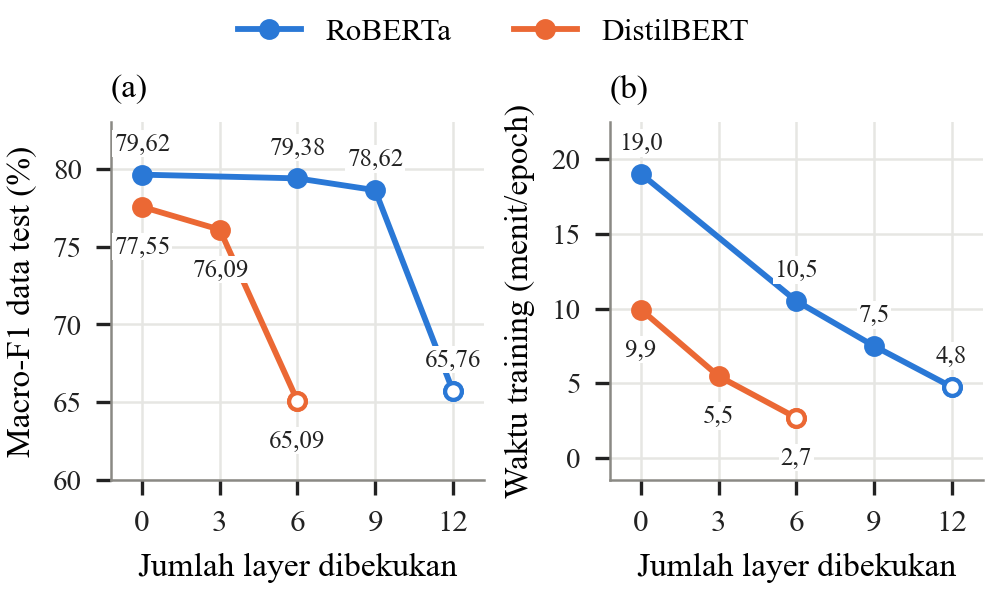
\includegraphics[width=\columnwidth]{fig_layer_dibekukan}
\caption{Macro-F1 data uji menurut jumlah layer yang dibekukan pada early fusion. Angka di bawah sumbu menunjukkan waktu training per epoch. Batang abu-abu adalah model yang seluruh layernya dibekukan (satu seed); batang lain adalah rata-rata tiga seed.}
\label{fig:frozen}
\end{figure}

\subsection{Pengaruh Parent Comment}
Friedman test menunjukkan perbedaan macro-F1 di antara ketiga input ($p = 0{,}009$, $W = 0{,}78$). Seperti terlihat pada Gambar~\ref{fig:input}, parent menaikkan macro-F1 kedua model, yaitu 1,10 dan 0,69 poin dengan early fusion serta 0,78 dan 0,72 poin dengan late fusion pada RoBERTa dan DistilBERT. Keempat kenaikan signifikan menurut paired t-test dan McNemar. Tambahan biaya early fusion kecil: waktu training hanya 1,15--1,16 kali, latensi batch 1 dan memori hampir tetap, dan hanya latensi per contoh pada batch 32 yang naik sekitar dua kali.

\begin{figure}[t]
\centering
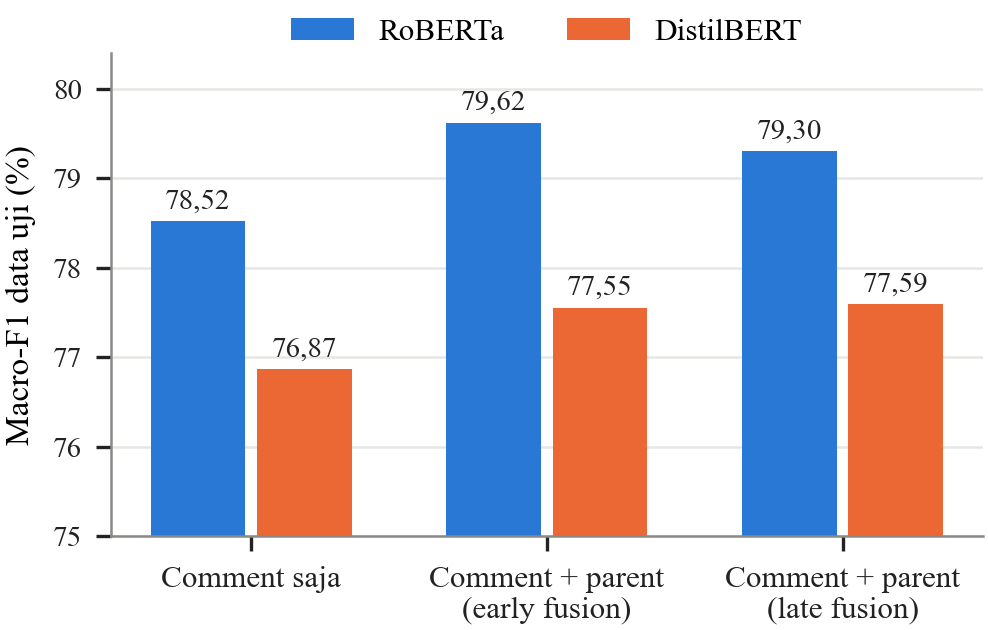
\includegraphics[width=\columnwidth]{fig_macro_f1_input}
\caption{Macro-F1 data uji untuk setiap model dan konfigurasi input (rata-rata tiga seed). Sumbu vertikal dimulai dari 75\% agar selisih antarkonfigurasi terlihat.}
\label{fig:input}
\end{figure}

Manfaat parent tidak merata. Pada 10.737 comment yang membuat model comment saja RoBERTa ragu, early fusion menaikkan macro-F1 RoBERTa sebesar 8,18 poin, tetapi hanya 0,25 poin pada comment yang diprediksi dengan yakin. Kenaikan pada comment 1--3 kata (2,59 poin) juga lebih besar daripada comment lebih dari 10 kata (0,71 poin), dan pada 5.886 comment (593 kalimat unik) yang muncul dengan label berbeda kenaikannya 2,73 poin. Meski begitu, parent memperbaiki rata-rata 6.236 prediksi RoBERTa per seed sekaligus merusak 5.119 prediksi lain.

\subsection{Strategi Fusion Terbaik}
Pada RoBERTa, early fusion unggul 0,32 poin dibanding late fusion (CI 95\% 0,15--0,49, $p_{\mathrm{Holm}} = 0{,}023$) dan juga signifikan menurut McNemar. Pada DistilBERT, keduanya setara (77,55\% dan 77,59\%), dan secara gabungan keunggulan early fusion tidak signifikan ($p_{\mathrm{Holm}} = 0{,}158$). Late fusion merupakan konfigurasi termahal, dengan waktu training sekitar 1,5 kali, memori 1,62--1,64 kali, dan latensi batch 1 sebesar 1,70--1,79 kali early fusion.

\section{Pembahasan}

\subsection{Trade-off antara RoBERTa dan DistilBERT}
RoBERTa terbukti lebih akurat, tetapi hanya 1,65--2,07 poin dengan biaya sekitar dua kali lipat, sehingga DistilBERT mempertahankan 97--98\% macro-F1 RoBERTa dengan kira-kira setengah sumber daya. Rasio biaya ini hampir sama pada ketiga input, sehingga kemungkinan besar ditentukan oleh ukuran model. RoBERTa cocok bila akurasi menjadi prioritas, misalnya analisis offline, sedangkan DistilBERT cocok bila latensi dan memori terbatas, seperti alat moderasi yang memproses comment terus-menerus.

\subsection{Pembekuan Layer dan Distilasi}
Jumlah layer yang dibekukan berpengaruh terhadap performa, tetapi tidak linear. Pembekuan separuh layer RoBERTa hanya mengurangi 0,24 poin, sementara waktu training turun 45\% dan memori 47\%, sejalan dengan \cite{ardakani2024slimfit}. Penurunan jelas baru terlihat pada 9 layer dan sangat besar bila semua layer dibekukan, sehingga representasi pralatih tetap perlu di-fine-tune. DistilBERT turun lebih cepat, kemungkinan karena layernya lebih sedikit. Pembekuan hanya menghemat biaya training sehingga cocok untuk model yang sering dilatih ulang, sedangkan DistilBERT menghemat biaya inferensi.

\subsection{Peran Parent Comment}
Parent terbukti meningkatkan performa kedua model, walaupun rata-rata hanya sekitar satu poin karena sebagian besar comment sudah dapat dipahami dari isinya sendiri. Peran parent terasa saat comment ambigu, misalnya balasan ``;)'' yang muncul 68 kali di data uji dan hanya enam yang sarkas. Sebagai balasan untuk ``Sarcasm doesn't translate well through text. Haha'' comment ini sarkas, tetapi untuk ``What is your Guilty Pleasure?'' tidak, padahal tanpa parent model pasti memberi prediksi yang sama. Kenaikan ini jauh lebih kecil daripada laporan Dubey dkk.\ (7,1 poin \cite{dubey2026efficient} dan 6,8 poin \cite{dubey2025unpacking}) yang memakai 7.370 sampel tanpa tanda baca dan huruf kapital, kondisi yang mungkin membuat model lebih bergantung pada parent.

\subsection{Early Fusion dan Late Fusion}
Early fusion dipilih sebagai strategi terbaik karena lebih akurat pada RoBERTa, setara pada DistilBERT, dan jauh lebih murah. Pada early fusion, token comment dapat memperhatikan kata tertentu di parent di setiap layer, sedangkan pada late fusion kedua teks diringkas dulu menjadi vektor. Karena sarkasme sering bergantung pada frasa tertentu di parent, late fusion kurang menguntungkan, meskipun mungkin berguna bila satu parent dibalas banyak comment.

\subsection{Perbandingan dengan Penelitian Lain dan Keterbatasan}
Skor yang lebih tinggi pada \cite{dubey2026efficient} (F1 95,6\%) dan \cite{zhang2025enhancing} (0,917) diperoleh dengan ukuran data, prapemrosesan, dan protokol evaluasi yang berbeda, dan tidak ada yang menyebutkan apakah potongan ``/s'' (Bagian~\ref{sec:data}) dibuang. Rasio biayanya justru sejalan: waktu training RoBERTa pada SARC di \cite{dubey2026efficient} 1,76 kali DistilBERT (8,1 dan 4,6 jam), sedangkan di sini 1,92--1,94 kali.

Penelitian ini memiliki beberapa keterbatasan. Pertama, training dibatasi tiga epoch, padahal 24 dari 29 run final mencapai skor validasi terbaik pada epoch terakhir. Kedua, hanya satu dataset dipakai dan labelnya berasal dari penanda ``/s'', sehingga comment sarkas tanpa penanda tercatat bukan sarkas \cite{khodak2018sarc}. Ketiga, model yang dibekukan memakai learning rate fine-tuning penuh, model beku penuh hanya memakai satu seed, dan setiap uji per konfigurasi hanya memiliki tiga pasangan. Terakhir, large language model tidak disertakan dan efisiensi hanya diukur pada satu GPU.

\section{Kesimpulan}
RoBERTa terbukti lebih akurat daripada DistilBERT dalam deteksi sarkasme pada SARC, tetapi keunggulannya hanya sekitar dua poin macro-F1 dengan biaya komputasi kira-kira dua kali lipat. Jumlah layer yang dibekukan memengaruhi performa, namun setengah layer RoBERTa dapat dibekukan dengan penurunan sangat kecil untuk menghemat biaya training. Parent comment meningkatkan performa kedua model, dan early fusion menjadi strategi terbaik karena paling akurat pada RoBERTa dan lebih hemat daripada late fusion. RoBERTa dengan early fusion disarankan bila akurasi menjadi prioritas, sedangkan DistilBERT dengan early fusion cocok bila latensi dan memori terbatas. Penelitian selanjutnya dapat memperpanjang training, mencari learning rate khusus untuk model yang dibekukan, menguji dataset lain, dan membandingkan dengan large language model.

\bibliographystyle{IEEEtran}
\bibliography{references}

\end{document}
